\renewcommand{\theequation}{\theenumi}
%\subsection{Problem}

\begin{enumerate}[label=\arabic*.,ref=\thesection.\theenumi]
\numberwithin{equation}{enumi}

\item A single variable function $f$ is said to be convex if
%
\begin{align}
\label{eq:convex_def}
f\sbrak{t x + \brak{1-t}y} \leq t f\brak{x} + \brak{1-t}f\brak{y}, 
\end{align}
%
for $\quad 0 < t < 1$.


\item
The following python script plots 
%
\begin{align}
f(\lambda) = a\lambda^2 + b\lambda + d
\end{align}
%
for 
\begin{align}
a &= \norm{\vec{m}}^2 > 0
\\
b &= \vec{m}^T\brak{\vec{A} -\vec{P}} 
\\
c &= \norm{\vec{A} -\vec{P}}^2
\end{align}
in Fig. \ref{fig:conv_def}.

Modify the above python script as follows to plot the parabola $f(x) = x^2$. Is it convex or concave?

\begin{lstlisting}
codes/optimization/1.2.py
\end{lstlisting}
%

%
%\begin{lstlisting}[language=sh]
%codes/optimization/1.1.py
%\end{lstlisting}
%%
\begin{figure}[!ht]
\centering
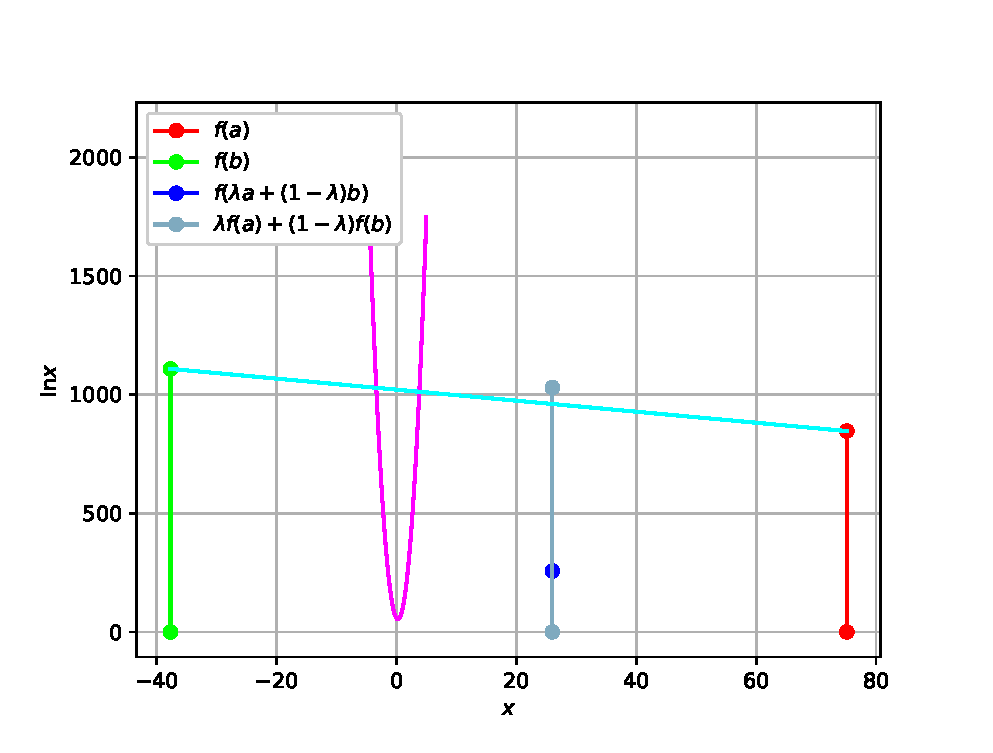
\includegraphics[width=\columnwidth]{./figs/convex.eps}
\caption{ $f(\lambda)$ versus $\lambda$}.
\label{fig:conv_def}	
\end{figure}
%
%\begin{figure}[!ht]
%\centering
%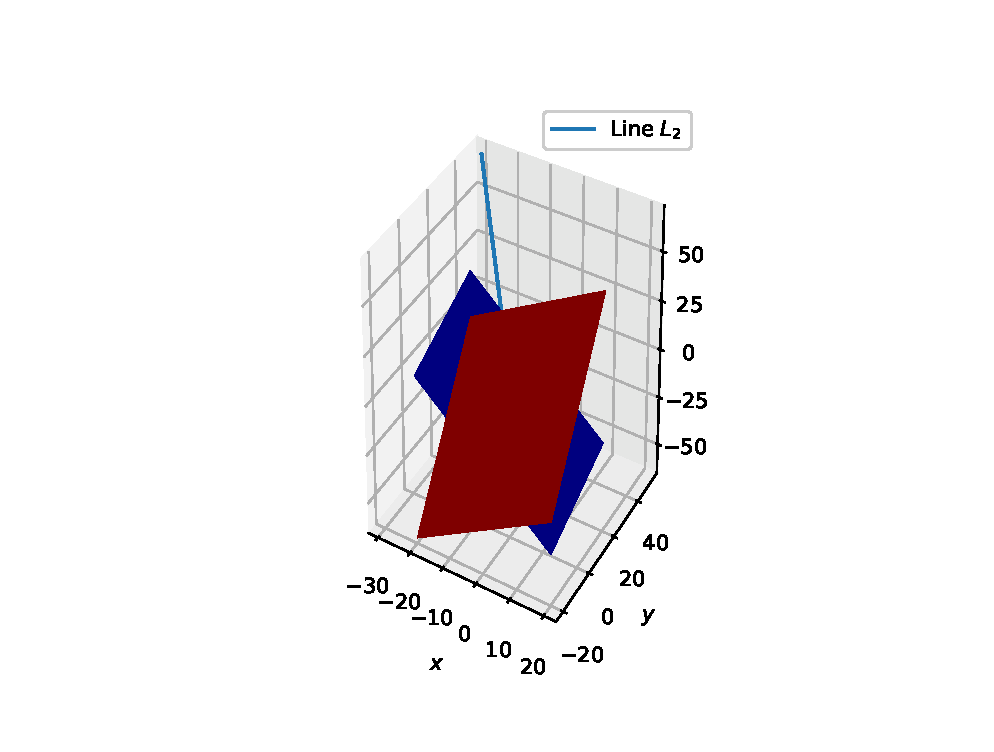
\includegraphics[width=\columnwidth]{./optimization/figs/1.2.eps}
%\caption{ $x^2$ versus $x$}.
%\label{fig.1.2}	
%\end{figure}
%
\item
Execute the following script to obtain Fig. \ref{fig.1.3}. Comment.

%
\begin{lstlisting}
codes/optimization/1.3.py
\end{lstlisting}

%
%\begin{figure}[!ht]
%\centering
%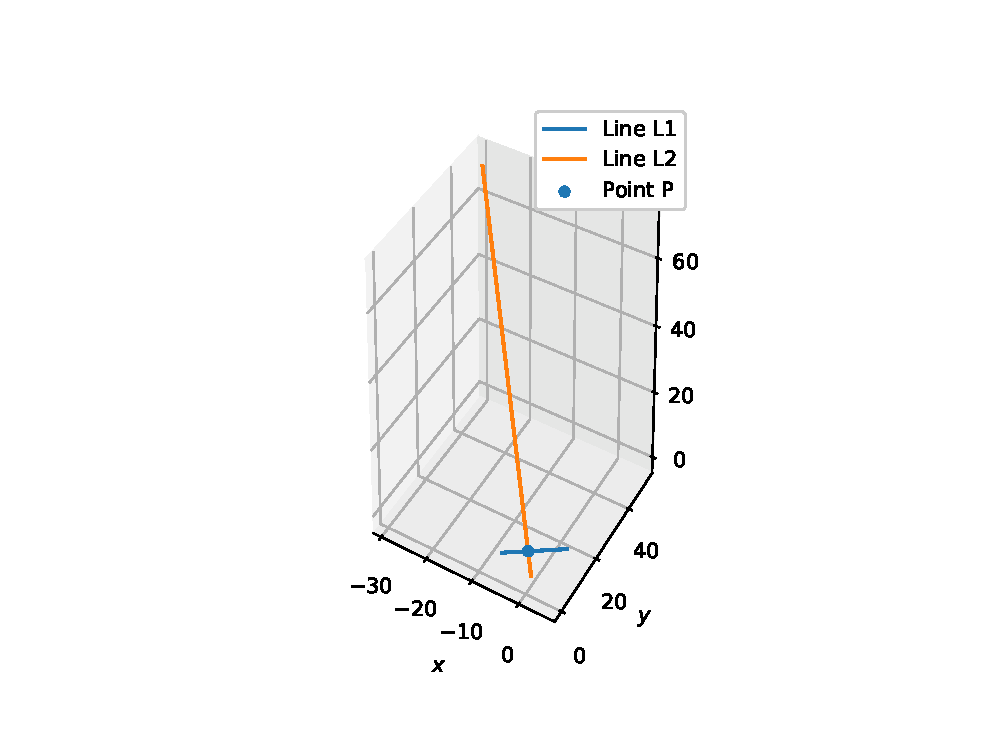
\includegraphics[width=\columnwidth]{./optimization/figs/1.3.eps}
%\caption{ Segments are below the curve}.
%\label{fig.1.3}	
%\end{figure}
%
\item
Modify the script in the previous problem for $f(x) = x^2$.  What can you conclude?

\item
Let 
\begin{equation}
f(\mathbf{x}) = x_1x_2, \quad \mathbf{x} \in \mathbf{R}^2
\end{equation}
Sketch $f(\mathbf{x})$ and deduce whether it is convex.
\item Show that 
\begin{equation}
f(\mathbf{x}) = \vec{x}^T\vec{V}\vec{x} 
\end{equation}
%
and find $\vec{V}$.
\item Show that 
\begin{equation}
\frac{1}{2}\nabla^2f(\mathbf{x}) = \vec{V}
\end{equation}

\item Use \eqref{eq:convex_def} to examine the convexity of $f(\vec{x})$.
\item How can you deduce the convexity of $f(\vec{x})$ using the eigenvalues of $\vec{V}$?
\item Show that $\vec{D}$ lies inside $\triangle ABC$ iff
\begin{align}
\vec{D} = \lambda_1\vec{A} + \lambda_2\vec{B} + \lambda_3\vec{C}
\end{align}
such that
\begin{align}
0 \le \lambda_1, \lambda_2, \lambda_3 &\le 1,
\\
0 \le \lambda_1+\lambda_2+\lambda_3 &\le 1,
\end{align}
\item Prove that the point $\myvec{4\\4}$ lies outside the triangle whose sides are the lines
\begin{align}
\myvec{3&4} \vec{x}&= 24
\\
\myvec{ 5 & - 3} \vec{x}&= 15
\\
\myvec{0 &1} \vec{x}&= 0
\end{align}


\end{enumerate}
%
